\documentclass[UTF8]{ctexart}
\usepackage{amsmath,amssymb}
\usepackage{fancyhdr}
\usepackage{amsmath,bm}
\usepackage{mathrsfs}
\usepackage{ntheorem}
\usepackage{graphicx}
\usepackage{subfigure}
\usepackage[top=2cm, bottom=2cm, left=2cm, right=2cm]{geometry}  
\usepackage{algorithm}  
\usepackage{algorithmicx}  
\usepackage{algpseudocode}
\usepackage{multirow}
\usepackage{tikz}
\usetikzlibrary{automata, positioning, arrows}
\tikzset{
    ->,
    >=stealth,
    node distance = 3cm,
    every state/.style={thick, fill=gray!10},
    initial text=$ $
}

\floatname{algorithm}{算法}  
\renewcommand{\algorithmicrequire}{\textbf{输入:}}  
\renewcommand{\algorithmicensure}{\textbf{输出:}}  
  
\theorembodyfont{\normalfont\rm\CJKfamily{song}}
%\theoremstyle{break}
\newtheorem{theorem}{定理}
\newtheorem{lemma}{引理}
\newtheorem{proposition}{命题}
\newtheorem*{proof}{证}[section]
\newtheorem*{solution}{解}[section]
\title{词法分析作业}
\author{丁元杰 17231164}
\date{\today}

\begin{document}
\maketitle

\section*{11.1}
\subsection*{(1)}
设$A$的正则集合是$L$,则$A\big| A$的正则集合是$L\cup L=L$,所以
$$A\big| A = A$$

\subsection*{(2)}
设$A$的正则集合为$L$,则$A^*$的正则集合是
$$L^*=\bigcup_{i\geq 0}{L^i}$$
那么$(A^*)^*$的正则集合就是
\begin{align*}
    (L^*)^*
    &=\bigcup_{j\geq 0}{\left(\bigcup_{i\geq 0}{L^i}\right)^j}\\
    &=\bigcup_{j\geq 0}{\bigcup_{i_0, i_1, \dots, i_j\geq 0}{L^{i_0+i_1+\cdots+i_j}}}\\
    &=\bigcup_{j\geq 0}{L^*}\\
    &=L^*
\end{align*}
从而有
$$(A^*)^*=A^*$$

\subsection*{(3)}
设$A$的正则集合为$L$,则$A^*$的正则集合是
$$L^*=\bigcup_{i\geq 0}{L^i}$$
那么$\varepsilon\big|AA^*$的正则集合就是
\begin{align*}
    L'
    &=\{\varepsilon\}\cup L\times\bigcup_{i\geq 0}{L^i}\\
    &=\{\varepsilon\}\cup\bigcup_{i\geq 1}{L^i}\\
    &=L^0\cup\bigcup_{i\geq 1}{L^i}\\
    &=\bigcup_{i\geq 0}{L^i} = L^*
\end{align*}
从而有
$$A*=\varepsilon\big|AA^*$$

\subsection*{(4)}
设$A$的正则集合为$L_a$,$B$的正则集合为$L_b$,则$(AB)^*A$的正则集合为
$$L_1=\bigcup_{i\geq 0}{(L_aL_b)^i}\times L_a$$
同理,$A(BA)^*$的正则集合为
$$L_2=L_a\times \bigcup_{i\geq 0}{(L_bL_a)^i}$$
那么
\begin{align*}
    L_1
    &=\left(\bigcup_{i\geq 0}{(L_aL_b)^i}\right)\times L_a\\
    &=\bigcup_{i\geq 0}{\left((L_aL_b)^i\times L_a\right)}\\
    &=\bigcup_{i\geq 0}{L_a\times (L_bL_a)^i}\\
    &=L_a\times \bigcup_{i\geq 0}{(L_bL_a)^i}\\
    &=L_2
\end{align*}
从而有
$$(AB)^*A=(AB)^*A$$

\subsection*{(5)}
设$A$的正则集合为$L_a$,$B$的正则集合为$L_b$,则$(A\big| B)^*$的正则集合为
$$L_1=\bigcup_{i\geq 0}{(L_a\cup L_b)^i}$$
同理,$(A^*B^*)^*$的正则集合为
$$L_2=\bigcup_{i\geq 0}{\left(\bigcup_{j\geq 0}{L_a^j}\times\bigcup_{j\geq 0}{L_b^j}\right)^i}$$
$(A^*\big|B^*)^*$的正则集合为
$$L_3=\bigcup_{i\geq 0}{\left(\bigcup_{j\geq 0}{L_a^j}\cup\bigcup_{j\geq 0}{L_b^j}\right)^i}$$
那么,先证$L_1\subseteq L_3$ \\
\begin{align*}
    &\Rightarrow L_a\subseteq L_a^*\text{ and } L_b\subseteq L_b^* \\
    &\Rightarrow L_a\cup L_b \subseteq L_a^*\cup L_b^* \\
    &\Rightarrow \bigcup_{i\geq 0}{(L_a\cup L_b)^i} \subseteq 
        \bigcup_{i\geq 0}{\left(\bigcup_{j\geq 0}{L_a^j}\cup\bigcup_{j\geq 0}{L_b^j}\right)^i} \\
    &\Rightarrow L_1\subseteq L_3
\end{align*}
再证$L_3\subseteq L_2$
\begin{align*}
    &\Rightarrow \{\varepsilon\}\subseteq L_a^*, L_b^* \\
    &\Rightarrow L_a^*, L_b^*\subseteq L_a^*\times L_b^* \\
    &\Rightarrow L_a^*\cup L_b^*\subseteq L_a^*\times L_b^* \\
    &\Rightarrow \bigcup_{i\geq 0}{\left(L_a^*\cup L_b^*\right)^i}
        \subseteq \bigcup_{i\geq 0}{\left(L_a^*\times L_b^*\right)^i} \\
    &\Rightarrow L_3\subseteq L_2
\end{align*}
最后证$L_2\subseteq L_1$
$$
\forall S\in L_2, \exists n_0 \geq 0\text{, s.t. }S\in \left(L_a^*\times L_b^*\right)^n_0
$$
那么可以将$S$写成如下形式:
$$
S=a_1b_1a_2b_2\dots a_{n_0}b_{n_0}\text{, where } a_{i}\in L_a^*\text{, and }b_{i}\in L_b^*, i=1, 2, \dots, n_0
$$
由于单位正则表达式$\varepsilon\in L_a^*, L_b^*$,满足$\varepsilon A=A\varepsilon = A$,所以将$a_i$与$b_i$中的$\varepsilon$选出,即可得到
$$
S=c_1c_2\dots c_l\text{, where }l \leq 2n_0 \text{, and } c_i\in L_a^+\text{ or }L_b^+, i=1,2,\dots,l
$$
更进一步地,$L_a^+$中的任意一个元素$s_a$均可以表示为$d_1d_2\dots d_k$,其中$d_i\in L_a, i=1,2,\dots,k$,对$L_b^+$同理 \\
所以原式最终可化为
$$
S=d_1^{(c_1)}d_2^{(c_1)}\dots d_{k_{c_1}}^{(c_1)}\dots d_l^{(c_l)}\dots d_{k_{c_l}}^{(c_l)}\text{, where } d_i^{(c_j)}\in L_a \text{ or } L_b 
$$
$$
\text{ i.e. } d_i^{(c_j)}\in L_a \cup L_b
$$
也即
$$S\in (L_a\cup L_b)^*$$
所以有
$$L_2\subseteq L_1$$

综上所述
$$L_1\subseteq L_3\subseteq L_2 \subseteq L_1$$
可以得到
$$L_1=L_2=L_3$$
即
$$(A\big| B)^*=(A^*B^*)^*=(A^*\big|B^*)^*$$

\section*{11.2}
\subsection*{(1)}
化简后的状态机
$$M=\left(\{s_0, s_1, s_2\}, \{0, 1\}, \delta, s_0, \{s_1, s_2\}\right)$$
状态转移参见\ref{DFM1}

\begin{table}[!htbp]
    \centering
    \begin{tabular}{|c|c|c|}
        \hline
        \multirow{2}*{状态}&\multicolumn{2}{c|}{输入}\\
        \cline{2-3}
        &$0$&$1$\\
        \hline
        $s_0$&$s_2$&$s_1$\\
        \cline{1-3}
        $s_1$&$s_1$&$s_1$\\
        \cline{1-3}
        $s_2$&$\emptyset$&$\emptyset$\\
        \hline
    \end{tabular}
    \label{DFM1}
    \caption{11.2(1)的状态机转移表}
\end{table}

\subsection*{(2)}
化简后的状态机
$$M=\left(\{1, 2, 3, 4, 5, 6, 7, 8, 9, 10, 11, 12, 13, 14, 15, 16\}, \{0, 1\}, \delta, 1, \{3, 7, 8, 10, 12\}\right)$$
状态转移参见\ref{DFM2}

\begin{table}
    \centering
    \begin{tabular}{|c|c|c|}
        \hline
        \multirow{2}*{状态}&\multicolumn{2}{c|}{输入}\\
        \cline{2-3}
        &$0$&$1$\\
        \hline
        1&-&2\\
        \cline{1-3}
        2&3&4\\
        \cline{1-3}
        3&-&-\\
        \cline{1-3}
        4&5&2\\
        \cline{1-3}
        5&-&6\\
        \cline{1-3}
        6&7&4\\
        \cline{1-3}
        7&8&9\\
        \cline{1-3}
        8&10&11\\
        \cline{1-3}
        9&12&9\\
        \cline{1-3}
        10&10&4\\
        \cline{1-3}
        11&13&2\\
        \cline{1-3}
        12&-&6\\
        \cline{1-3}
        13&14&6\\
        \cline{1-3}
        14&-&15\\
        \cline{1-3}
        15&16&-\\
        \cline{1-3}
        16&14&2\\
        \hline
    \end{tabular}
    \label{DFM2}
    \caption{11.2(2)的状态机转移表}
\end{table}

\subsection*{(3)}
$$M=\left(\{1, 2, 3, 4, 5\}, \{0, 1\}, \delta, 1, \{5\}\right)$$
状态转移参见\ref{DFM3}

\begin{table}
    \centering
    \begin{tabular}{|c|c|c|}
        \hline
        \multirow{2}*{状态}&\multicolumn{2}{c|}{输入}\\
        \cline{2-3}
        &$0$&$1$\\
        \hline
        1&-&2\\
        \cline{1-3}
        2&2&3\\
        \cline{1-3}
        3&4&3\\
        \cline{1-3}
        4&2&5\\
        \cline{1-3}
        5&4&3\\
        \cline{1-3}
        \hline
    \end{tabular}
    \label{DFM3}
    \caption{11.2(3)的状态机转移表}
\end{table}

\section*{11.4}
\subsection*{(a)}
确定化、最小化后如图\ref{DFA4}
\begin{figure}[ht] % ’ht’ tells LaTeX to place the figure ’here’ or at the top of the page
    \centering % centers the figure
    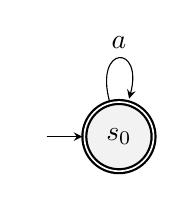
\begin{tikzpicture}
    % tikz code goes here
        \node[state, initial, accepting] (q1) {$s_0$};
        \draw (q1) edge[loop above] node{$a$} (q1);
    \end{tikzpicture}
    \caption{11.4(a) 状态图}
    \label{DFA4}
\end{figure}

\subsection*{(b)}
确定化、最小化后如图\ref{DFA5}
\begin{figure}[ht] % ’ht’ tells LaTeX to place the figure ’here’ or at the top of the page
    \centering % centers the figure
    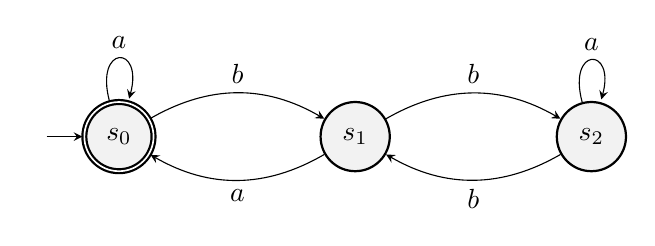
\begin{tikzpicture}
    % tikz code goes here
        \node[state, initial, accepting] (q1) {$s_0$};
        \node[state, right of=q1] (q2) {$s_1$};
        \node[state, right of=q2] (q3) {$s_2$};
        \draw (q1) edge[loop above] node{$a$} (q1)
            (q1) edge[bend left, above] node{$b$} (q2)
            (q2) edge[bend left, above] node{$b$} (q3)
            (q3) edge[loop above] node{$a$} (q3)
            (q3) edge[bend left, below] node{$b$} (q2)
            (q2) edge[bend left, below] node{$a$} (q1);

    \end{tikzpicture}
    \caption{11.4(b) 状态图}
    \label{DFA5}
\end{figure}

\section*{11.5}

确定化、最小化后如图\ref{DFA6}
\begin{figure}[ht] % ’ht’ tells LaTeX to place the figure ’here’ or at the top of the page
    \centering % centers the figure
    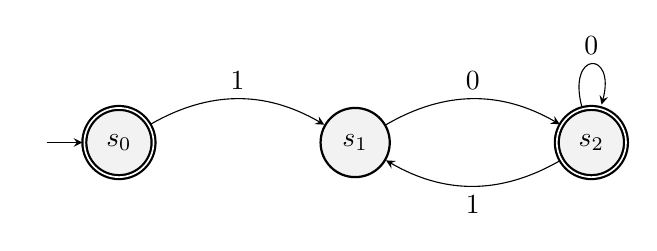
\begin{tikzpicture}
    % tikz code goes here
        \node[state, initial, accepting] (q1) {$s_0$};
        \node[state, right of=q1] (q2) {$s_1$};
        \node[state, accepting, right of=q2] (q3) {$s_2$};
        \draw
            (q1) edge[bend left, above] node{$1$} (q2)
            (q2) edge[bend left, above] node{$0$} (q3)
            (q3) edge[loop above] node{$0$} (q3)
            (q3) edge[bend left, below] node{$1$} (q2);

    \end{tikzpicture}
    \caption{11.4(b) 状态图}
    \label{DFA6}
\end{figure}

\end{document}